%!TEX root =../main-tokyo.tex
% ##################################################################################################################
\chapter{Joinville}
\label{ch:joinville}
\hfill \textbf{Authors:} Davi Guggisberg Bicudo, Gian Ricardo Berkenbrock

% ##################################################################################################################
Joinville \cite{pmj} is a mid-sized industrial city in the south of Brazil, with around 550\,000 inhabitants. It has a large workforce, including commuters from neighboring cities and an intense industrial activity profile,meaning that companies work often in three shifts, causing peculiar traffic patterns.  Many people also have 12-hour daily routines, encompassing work and higher education. 

The Joinville traffic model was built as an initial step of a project to simulate the entire northeast region of Santa Catarina state, including air traffic, shipping, state highways and neighboring cities. The project aims to build a complete data base of people and freight movement in the region. The first version of the urban Joinville model is now complete, produced as a graduate thesis at the Federal University of Santa Catarina (UFSC) \url{http://ufsc.br}, Transportation and Logistics Engineering course \url{http://transporteslogistica.joinville.ufsc.br}.%
\footnote{The authors would like to thank their sponsors Federal University of Santa Catarina (UFSC) and Urban Sustainable Planning Institute of Joinville (IPPUJ).} 

The scenario population was generated with data from the 2010~Brazilian census combined with demographic information from the city’s travel survey; travel demand was generated from the same survey. Both were designed to fit into the \gls{matsim}, using Tutorial classes (with some adaptations).

The network was produced with vector data provided by the local Urban Sustainable Planning Institute of Joinville (IPPUJ) \url{https://ippuj.joinville.sc.gov.br}. The data came as a shapefile, with numerous connectivity problems. We were able to fix them using scripts in Python with the \lstinline|NetworkX| module \cite{networkx}. Information was transforming  from vector data into a graph, addressing issues with the help of \gls{qgis} and finally writing as the \gls{matsim} \gls{xml} network format. The facilities were produced from land-use data provided by the city government.

For now, the model runs only with cars, using a full sample of the population. From the available data, we inferred 135\,652 agents traveling by car; the rest were removed from the simulation. Figure~\ref{fig:Joinville_ssMain} shows a screenshot of the Events using \gls{via}.

Figure~\ref{fig:Joinville_counts} shows the comparison between simulated and count data for 20\,links in the morning peak from 7 to 8\,AM. The count data available for comparison is still sparse and could not be used as effectively as we hoped; we know that calibration is needed for the next model versions. The good news is that the local authorities are installing more than a hundred counting stations throughout the city within the next couple of months and a new travel survey will be conducted this year. 

\createfigure%
{Screenshot of the simulation using \gls{via}}%
{Screenshot of the simulation using \gls{via}}%
{\label{fig:Joinville_ssMain}}%
{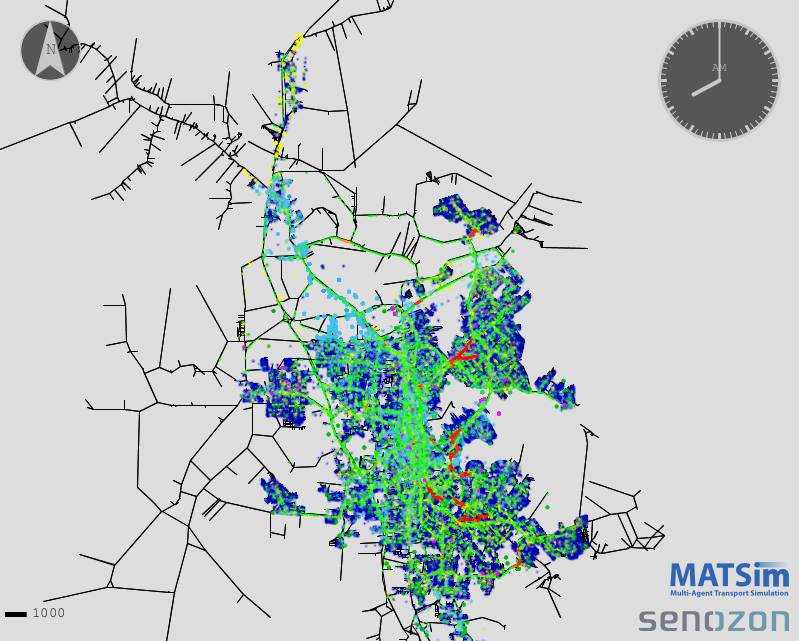
\includegraphics[width=0.7\textwidth, angle=0]{./scenarios/figures/Joinville_ssMain.png}}%
{}

\createfigure%
{Count comparisons for the morning peak at 7-8\,AM}%
{Count comparisons for the morning peak at 7-8\,AM}%
{\label{fig:Joinville_counts}}%
{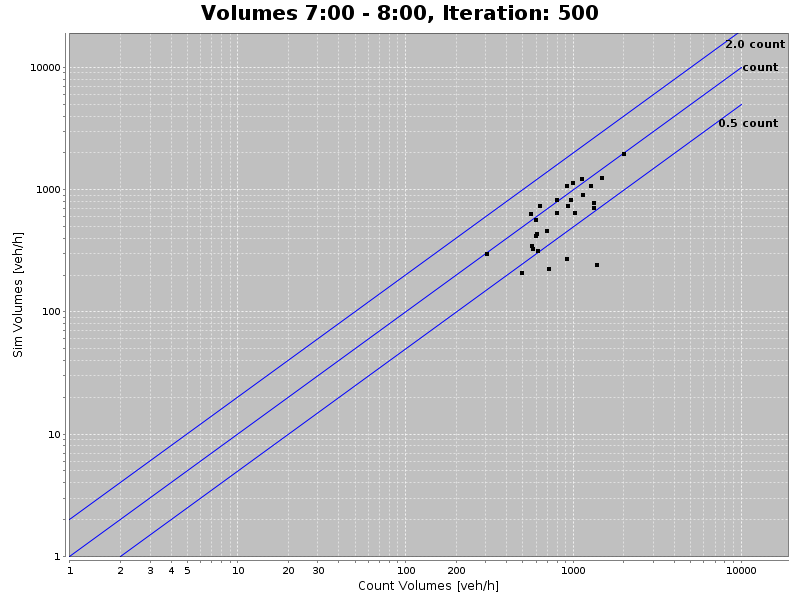
\includegraphics[width=0.7\textwidth, angle=0]{./scenarios/figures/Joinville_LogManha.png}}%
{}

% ##################################################################################################################

% Local Variables:
% mode: latex
% mode: reftex
% mode: visual-line
% TeX-master: "../main"
% comment-padding: 1
% fill-column: 9999
% End: 
